\clearpage

\subsection{Opaque without Survivability}\label{ILP_Opaque_Survivability}
\begin{tcolorbox}	
\begin{tabular}{p{2.75cm} p{0.2cm} p{10.5cm}} 	
\textbf{Student Name}  &:& Tiago Esteves    (October 03, 2017 - )\\
\textbf{Goal}          &:& Implement the ILP model for the opaque transport mode without survivability.
\end{tabular}
\end{tcolorbox}

\subsubsection{Model description}

First, for a better understanding of the functions and variables used in the ILP, a table \ref{description_opaque} will be created with all indexes, inputs and variables and with their respective description.\\

\begin{table}[h!]
\centering
\begin{tabular}{ |p{1cm}||p{13cm}|}
 \hline
 \multicolumn{2}{|c|}{Description of notation used in the objective function} \\
 \hline
 \hline
 $i$ & index for start node of a physical link \\
 $j$ & index for end node of a physical link \\
 $o$ & index for node that is origin of a demand \\
 $d$ & index for node that is destination of a demand \\
 $c$ & index for bit rate of the client signal \\
 $($ i,j $)$ & physical link between the nodes $i$ and $j$ \\
 $($ o,d $)$ & demand between the nodes $o$ and $d$ \\
 $C$ & set of the client signal \\
 $f_{ij}^{od}$ & binary variable indicating if link between the nodes $i$ and $j$ is used in the path between nodes $o$ and $d$ \\
 $L_{ij}$ & binary variable indicating if link between the nodes $i$ and $j$ is used \\
 $W_{ij}$ & number of optical channels between the nodes $i$ and $j$\\
 $B_c $ & client signals granularities $($1.25, 2.5, 10, 40, 100$)$ \\
 $D_{odc}$ & client demands with bit rate $c$ between nodes $o$ and $d$ \\
 $G_{ij}$ & network topology in form of adjacency matrix \\
 \hline
\end{tabular}
\caption{Table with description of variables}
\label{description_opaque}
\end{table}

Before carrying out the description of the objective function we must take into account the following particularity of this mode of transport:
\begin{itemize}
  \item $N_{OXC,n}$ = 0, \quad $\forall$ n
  \item $N_{EXC,n}$ = 1, \quad $\forall$ n that process traffic
\end{itemize}


\vspace{11pt}
The objective function of following the ILP is a minimization of the CAPEX through the equation \ref{Capex} where in this case for the cost of nodes we only have in consideration the electric cost \ref{Capex_Node_EXC} because of the particularity previously mentioned.
In this case the value of $P_{exc,c,n}$ is obtained by equation \ref{EXC_pexc1_opaque} for long-reach and by the equation \ref{EXC_pexc2_opaque} for short-reach.\\

\newpage
As previously mentioned, equation \ref{EXC_pexc1_opaque} refers to the number of long-reach ports, that is, the number of line ports of node n is calculated.

\begin{equation}
P_{exc,-1,n} = \sum_{j=1}^{N} w_{nj}
\label{EXC_pexc1_opaque}
\end{equation}

\begin{itemize}
\item{$P_{exc,-1,n}$	$\rightarrow$	Number of long-reach ports of the electrical switch, i.e. number of line ports}
\item{$w_{nj}$			$\rightarrow$	Number of optical channels between node $n$ and node $j$}
\end{itemize}

\vspace{11pt}
As previously mentioned, equation \ref{EXC_pexc2_opaque} refers to the number of sort-reach ports, that is, the number of tributary ports with bit-rate c in node n is calculated.

\begin{equation}
P_{exc,c,n} = \sum_{d=1}^{N} D_{nd,c}
\label{EXC_pexc2_opaque}
\end{equation}

\begin{itemize}
\item{$P_{exc,c,n}$	$\rightarrow$	Number of sort-reach ports of the electrical switch}
\item{$D_{nj,c}$	$\rightarrow$	client demands between nodes $n$ and $d$ with bit rate $c$}
\end{itemize}

\vspace{11pt}
In this case there is the following particularity:

\begin{itemize}
  \item When $n$=$j$ the value of client demands is always zero, i.e, $D_{nn,c}=0$
\end{itemize}


\vspace{17pt}
The objective function, to be minimized, is the expression \ref{ILPOpaque_CAPEX}.\\


$subject$ $to$
\begin{equation}
\sum_{j\textbackslash \{o\}} f_{ij}^{od} = 1  \qquad \qquad \qquad \qquad \qquad \qquad \qquad \qquad \qquad \qquad
\forall(o,d) : o < d, \forall i: i = o
\label{ILPOpaque1_Surv}
\end{equation}

This constraint are equal to the constraint \ref{ILPOpaque1_CAPEX} assuming that Z variable has the value of 1.

\begin{equation}
\sum_{j\textbackslash \{o\}} f_{ij}^{od} = \sum_{j\textbackslash \{d\}} f_{ji}^{od}   \qquad \qquad \qquad \qquad \qquad \qquad \qquad \qquad
\forall(o,d) : o < d, \forall i: i \neq o,d
\label{ILPOpaque2_Surv}
\end{equation}

This constraint are equal to the constraint \ref{ILPOpaque2_CAPEX}.

\begin{equation}
\sum_{j\textbackslash \{d\}} f_{ji}^{od} = 1  \qquad \qquad \qquad \qquad \qquad \qquad \qquad \qquad \qquad \qquad
\forall(o,d) : o < d, \forall i: i = d
\label{ILPOpaque3_Surv}
\end{equation}

This constraint are equal to the constraint \ref{ILPOpaque3_CAPEX} assuming that Z variable has the value of 1.

\begin{equation}
\sum_{(o,d):o<d} \left(f_{ij}^{od} + f_{ji}^{od}\right) + \sum_{c\in C} (B\left(c\right) D_{odc}\leq100 W_{ij} G_{ij} \qquad \qquad \qquad \qquad
\forall(i,j) : i < j
\label{ILPOpaque4_Surv}
\end{equation}

This restriction is considered grooming constraint, so it means the total client traffic flows can not be greater than the capacity of optical channels on all links.

\begin{equation}
W_{ij} \leq K_{ij} L_{ij} \qquad  \qquad \qquad \qquad \qquad \qquad \qquad \qquad \qquad \qquad \qquad \qquad \forall(i,j) : i < j
\label{ILPOpaque5_Surv}
\end{equation}

This restriction concerns the capacity of the optical channels which must be less or equal to the maximum number of optical channels. For any situation the maximum number of optical channels supported by each transmission system is 80, i.e., $K_{ij}$ = 80.

\begin{equation}
f_{ij}^{od} , f_{ji}^{od} \in \{0,1\}   \qquad \qquad \qquad \qquad \qquad \qquad \qquad \qquad \qquad
\forall(i,j) : i < j, \forall(o,d) : o < d
\label{ILPOpaque6_Surv}
\end{equation}

The number of flows per demand in this case can be zero if there are no traffic demands or one if considering traffic.

\begin{equation}
W_{ij} \in \mathbb{N}  \qquad \qquad \qquad \qquad \qquad \qquad \qquad \qquad \qquad \qquad \qquad \qquad \qquad
\forall(i,j) : i < j
\label{ILPOpaque7_Surv}
\end{equation}

The last constraint is just needed to ensure the number optical of channels is a positive integer values greater than zero.\\


\subsubsection{Result description}

To perform the calculations using the implementation of the models described in previous subsection it is necessary to use a mathematical software tool. For this we will use MATLAB which is ideal for dealing with linear programming problems and can call the LPsolve through an external interface.\\
We already have all the necessary to obtain the CAPEX value for the reference network \ref{Reference_Network_Topology}. As described in the subsection of network traffic \ref{Reference_Network_Traffic}, we have three values of network traffic (low, medium and high traffic) so we have to obtain three different CAPEX.
The value of the CAPEX of the network will be calculated based on the costs of the equipment present in the table \ref{table_cost_ilp}.

\newpage
\textbf{Low Traffic Scenario:}\\

In this scenario we have to take into account the traffic calculated in \ref{low_traffic_scenario}. In table \ref{link_opaque_surv_ref_low} we can see the number of optical channels and the number of amplifiers for each link calculated through MatLab.

\begin{table}[h!]
\centering
\begin{tabular}{|| c | c | c ||}
 \hline
 \multicolumn{3}{|| c ||}{Information regarding LINK} \\
 \hline
 \hline
 Bidirectional Link & Optical Channels & Amplifiers\\
 \hline
 Node 1 <-> Node 2 & 1 & 4 \\
 Node 1 <-> Node 3 & 1 & 6 \\
 Node 2 <-> Node 3 & 1 & 0 \\
 Node 2 <-> Node 4 & 2 & 6 \\
 Node 3 <-> Node 5 & 1 & 8 \\
 Node 4 <-> Node 5 & 1 & 1 \\
 Node 4 <-> Node 6 & 2 & 7 \\
 Node 5 <-> Node 6 & 2 & 3 \\
 \hline
\end{tabular}
\caption{Table with information regarding Link}
\label{link_opaque_surv_ref_low}
\end{table}

In table \ref{node_opaque_surv_ref_low}  we can see the number of transceivers, the number of line ports and the number of tributary ports for each node.

\begin{table}[h!]
\centering
\begin{tabular}{|| c | c | c | c ||}
 \hline
 \multicolumn{4}{|| c ||}{Information regarding NODE} \\
 \hline
 \hline
 Node & Transceiver & Line Ports & Tributary Ports\\
 \hline
 1 & 2 & 2 & 29 \\
 2 & 3 & 4 & 23 \\
 3 & 3 & 3 & 18 \\
 4 & 3 & 5 & 20 \\
 5 & 3 & 4 & 24 \\
 6 & 2 & 4 & 22 \\
\hline
\end{tabular}
\caption{Table with information regarding Node}
\label{node_opaque_surv_ref_low}
\end{table}

Through the information obtained previously on the nodes we can now create tables with detailed information about each node.\\

\begin{table}[h!]
\centering
\begin{tabular}{|| c | c ||}
 \hline
 \multicolumn{2}{|| c ||}{Detailed description of Node 1} \\
 \hline
 \hline
 \multirow{2}{*}{2 transceivers} & One to connect to Node 2 \\
  & One to connect to Node 3 \\ \hline
\multirow{2}{*}{2 line ports} & 1 line ports to connect to Node 2 \\
 & 1 line ports to connect to Node 3 \\ \hline
\multirow{3}{*}{29 tributary ports} & where 13 is the ODU0 \\
 & where 13 is the ODU1 \\
 & where 3 is the ODU2 \\
\hline
\end{tabular}
\caption{Table with detailed description of node 1}
\end{table}


\begin{table}[h!]
\centering
\begin{tabular}{|| c | c ||}
 \hline
 \multicolumn{2}{|| c ||}{Detailed description of Node 2} \\
 \hline
 \hline
 \multirow{3}{*}{3 transceivers} & One to connect to Node 1 \\
  & One to connect to Node 3 \\
  & One to connect to Node 4 \\ \hline
\multirow{3}{*}{4 line ports} & 1 line ports to connect to Node 1 \\
 & 1 line ports to connect to Node 3 \\
 & 2 line ports to connect to Node 4 \\ \hline
\multirow{5}{*}{23 tributary ports} & where 11 is the ODU0 \\
 & where 7 is the ODU1 \\
 & where 2 is the ODU2 \\
 & where 2 is the ODU3 \\
 & where 1 is the ODU4 \\
\hline
\end{tabular}
\caption{Table with detailed description of node 2}
\end{table}

\newpage
\begin{table}[h!]
\centering
\begin{tabular}{|| c | c ||}
 \hline
 \multicolumn{2}{|| c ||}{Detailed description of Node 3} \\
 \hline
 \hline
 \multirow{3}{*}{3 transceivers} & One to connect to Node 1 \\
  & One to connect to Node 2 \\
  & One to connect to Node 5 \\ \hline
\multirow{3}{*}{3 line ports} & 1 line ports to connect to Node 1 \\
 & 1 line ports to connect to Node 2 \\
 & 1 line ports to connect to Node 5 \\ \hline
\multirow{4}{*}{18 tributary ports} & where 7 is the ODU0 \\
 & where 6 is the ODU1\\
 & where 3 is the ODU2\\
 & where 2 is the ODU3\\
\hline
\end{tabular}
\caption{Table with detailed description of node 3}
\end{table}

\begin{table}[h!]
\centering
\begin{tabular}{|| c | c ||}
 \hline
 \multicolumn{2}{|| c ||}{Detailed description of Node 4} \\
 \hline
 \hline
 \multirow{3}{*}{3 transceivers} & One to connect to Node 2 \\
 & One to connect to Node 5 \\
 & One to connect to Node 6 \\ \hline
\multirow{3}{*}{5 line ports} & 2 line ports to connect to Node 2 \\
 & 1 line ports to connect to Node 5 \\
 & 2 line ports to connect to Node 6 \\ \hline
\multirow{3}{*}{20 tributary ports} & where 7 is the ODU0 \\
 & where 10 is the ODU1 \\
 & where 3 is the ODU2 \\
\hline
\end{tabular}
\caption{Table with detailed description of node 4}
\end{table}

\newpage
\begin{table}[h!]
\centering
\begin{tabular}{|| c | c ||}
 \hline
 \multicolumn{2}{|| c ||}{Detailed description of Node 5} \\
 \hline
 \hline
 \multirow{3}{*}{3 transceivers} & One to connect to Node 3 \\
 & One to connect to Node 4 \\
 & One to connect to Node 6 \\ \hline
\multirow{3}{*}{4 line ports} & 1 line ports to connect to Node 3 \\
 & 1 line ports to connect to Node 4 \\
 & 2 line ports to connect to Node 6 \\ \hline
\multirow{5}{*}{24 tributary ports} & where 14 is the ODU0 \\
 & where 4 is the ODU1 \\
 & where 4 is the ODU2 \\
 & where 1 is the ODU3 \\
 & where 1 is the ODU4 \\
\hline
\end{tabular}
\caption{Table with detailed description of node 5}
\end{table}

\begin{table}[h!]
\centering
\begin{tabular}{|| c | c ||}
 \hline
 \multicolumn{2}{|| c ||}{Detailed description of Node 6} \\
 \hline
 \hline
 \multirow{2}{*}{2 transceivers} & One to connect to Node 4 \\
  & One to connect to Node 5 \\ \hline
\multirow{2}{*}{4 line ports} & 2 line ports to connect to Node 4 \\
 & 2 line ports to connect to Node 5 \\ \hline
\multirow{5}{*}{22 tributary ports} & where 8 is the ODU0 \\
 & where 10 is the ODU1 \\
 & where 1 is the ODU2 \\
 & where 1 is the ODU3 \\
 & where 2 is the ODU4 \\
\hline
\end{tabular}
\caption{Table with detailed description of node 6}
\end{table}


Now let's focus on the path information. These paths are bidirectional paths so the path from one node to another is the same path in the opposite direction. In table \ref{path_opaque_surv_ref_low} we can see all the paths obtained for all nodes.\\

\begin{table}[h!]
\centering
\begin{tabular}{|| c | c ||}
 \hline
 \multicolumn{2}{|| c ||}{Information regarding PATHS} \\
 \hline
 \hline
 Node1 <-> Node2 & -Link(1,2) \\
 Node1 <-> Node3 & -Link(1,3) \\
 Node1 <-> Node4 & -Link(1,2) -Link(2,4)\\
 Node1 <-> Node5 & -Link(1,3) -Link(3,5)\\
 Node1 <-> Node6 & -Link(1,3) -Link(3,5) -Link(5,6)\\
 Node2 <-> Node3 & -Link(2,3)\\
 Node2 <-> Node4 & -Link(2,4)\\
 Node2 <-> Node5 & -Link(2,3) -Link(3,5)\\
 Node2 <-> Node6 & -Link(2,4) -Link(4,6)\\
 Node3 <-> Node4 & -Link(3,2) -Link(2,4)\\
 Node3 <-> Node5 & -Link(3,5)\\
 Node3 <-> Node6 & -Link(3,5) -Link(5,6)\\
 Node4 <-> Node5 & -Link(4,5)\\
 Node4 <-> Node6 & -Link(4,6)\\
 Node5 <-> Node6 & -Link(5,6)\\
 \hline
\end{tabular}
\caption{Table with description of path}
\label{path_opaque_surv_ref_low}
\end{table}


Finally, through the figure \ref{scriptopaque_surv_ref_low} we can see the result of CAPEX obtained with this ILP model.

\begin{figure}[h!]
\centering
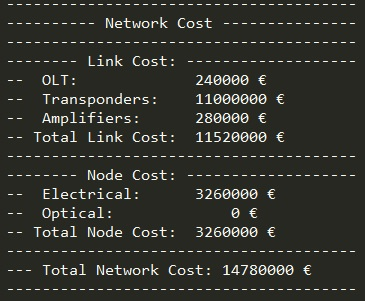
\includegraphics[width=9cm]{sdf/ilp/opaque_survivability/figures/script_opaque_surv_ref_low}
\caption{The ILP script used in the low scenario with the network cost.}
\label{scriptopaque_surv_ref_low}
\end{figure}

As we can see the cost of CAPEX for this scenario is \textbf{14 780 000 \euro}.\\


\textbf{Medium Traffic Scenario:}\\

In this scenario we have to take into account the traffic calculated in \ref{medium_traffic_scenario}. In table \ref{link_opaque_surv_ref_medium} we can see the number of optical channels and the number of amplifiers for each link calculated through MatLab.

\begin{table}[h!]
\centering
\begin{tabular}{|| c | c | c ||}
 \hline
 \multicolumn{3}{|| c ||}{Information regarding LINK} \\
 \hline
 \hline
 Bidirectional Link & Optical Channels & Amplifiers\\
 \hline
 Node 1 <-> Node 2 & 4 & 4 \\
 Node 1 <-> Node 3 & 4 & 6 \\
 Node 2 <-> Node 3 & 4 & 0 \\
 Node 2 <-> Node 4 & 19 & 6 \\
 Node 3 <-> Node 5 & 9 & 8 \\
 Node 4 <-> Node 5 & 5 & 1 \\
 Node 4 <-> Node 6 & 16 & 7 \\
 Node 5 <-> Node 6 & 14 & 3 \\
 \hline
\end{tabular}
\caption{Table with information regarding Link}
\label{link_opaque_surv_ref_medium}
\end{table}

In table \ref{node_opaque_surv_ref_medium}  we can see the number of transceivers, the number of line ports and the number of tributary ports for each node.

\begin{table}[h!]
\centering
\begin{tabular}{|| c | c | c | c ||}
 \hline
 \multicolumn{4}{|| c ||}{Information regarding NODE} \\
 \hline
 \hline
 Node & Transceiver & Line Ports & Tributary Ports\\
 \hline
 1 & 2 & 8 & 290 \\
 2 & 3 & 27 & 230 \\
 3 & 3 & 17 & 180 \\
 4 & 3 & 40 & 200 \\
 5 & 3 & 28 & 240 \\
 6 & 2 & 30 & 220 \\
\hline
\end{tabular}
\caption{Table with information regarding Node}
\label{node_opaque_surv_ref_medium}
\end{table}

Through the information obtained previously on the nodes we can now create tables with detailed information about each node.\\

\newpage
\begin{table}[h!]
\centering
\begin{tabular}{|| c | c ||}
 \hline
 \multicolumn{2}{|| c ||}{Detailed description of Node 1} \\
 \hline
 \hline
 \multirow{2}{*}{2 transceivers} & One to connect to Node 2 \\
  & One to connect to Node 3 \\ \hline
\multirow{2}{*}{8 line ports} & 4 line ports to connect to Node 2 \\
 & 4 line ports to connect to Node 3 \\ \hline
\multirow{3}{*}{290 tributary ports} & where 130 is the ODU0 \\
 & where 130 is the ODU1 \\
 & where 30 is the ODU2 \\
\hline
\end{tabular}
\caption{Table with detailed description of node 1}
\end{table}


\begin{table}[h!]
\centering
\begin{tabular}{|| c | c ||}
 \hline
 \multicolumn{2}{|| c ||}{Detailed description of Node 2} \\
 \hline
 \hline
 \multirow{3}{*}{3 transceivers} & One to connect to Node 1 \\
  & One to connect to Node 3 \\
  & One to connect to Node 4 \\ \hline
\multirow{3}{*}{27 line ports} & 4 line ports to connect to Node 1 \\
 & 4 line ports to connect to Node 3 \\
 & 19 line ports to connect to Node 4 \\ \hline
\multirow{5}{*}{230 tributary ports} & where 110 is the ODU0 \\
 & where 70 is the ODU1 \\
 & where 20 is the ODU2 \\
 & where 20 is the ODU3 \\
 & where 10 is the ODU4 \\
\hline
\end{tabular}
\caption{Table with detailed description of node 2}
\end{table}


\begin{table}[h!]
\centering
\begin{tabular}{|| c | c ||}
 \hline
 \multicolumn{2}{|| c ||}{Detailed description of Node 3} \\
 \hline
 \hline
 \multirow{3}{*}{3 transceivers} & One to connect to Node 1 \\
  & One to connect to Node 2 \\
  & One to connect to Node 5 \\ \hline
\multirow{3}{*}{17 line ports} & 4 line ports to connect to Node 1 \\
 & 4 line ports to connect to Node 2 \\
 & 9 line ports to connect to Node 5 \\ \hline
\multirow{4}{*}{180 tributary ports} & where 70 is the ODU0 \\
 & where 60 is the ODU1\\
 & where 30 is the ODU2\\
 & where 20 is the ODU3\\
\hline
\end{tabular}
\caption{Table with detailed description of node 3}
\end{table}

\newpage
\begin{table}[h!]
\centering
\begin{tabular}{|| c | c ||}
 \hline
 \multicolumn{2}{|| c ||}{Detailed description of Node 4} \\
 \hline
 \hline
 \multirow{3}{*}{3 transceivers} & One to connect to Node 2 \\
 & One to connect to Node 5 \\
 & One to connect to Node 6 \\ \hline
\multirow{3}{*}{40 line ports} & 19 line ports to connect to Node 2 \\
 & 5 line ports to connect to Node 5 \\
 & 16 line ports to connect to Node 6 \\ \hline
\multirow{3}{*}{200 tributary ports} & where 70 is the ODU0 \\
 & where 100 is the ODU1 \\
 & where 30 is the ODU2 \\
\hline
\end{tabular}
\caption{Table with detailed description of node 4}
\end{table}


\begin{table}[h!]
\centering
\begin{tabular}{|| c | c ||}
 \hline
 \multicolumn{2}{|| c ||}{Detailed description of Node 5} \\
 \hline
 \hline
 \multirow{3}{*}{3 transceivers} & One to connect to Node 3 \\
 & One to connect to Node 4 \\
 & One to connect to Node 6 \\ \hline
\multirow{3}{*}{28 line ports} & 9 line ports to connect to Node 3 \\
 & 5 line ports to connect to Node 4 \\
 & 14 line ports to connect to Node 6 \\ \hline
\multirow{5}{*}{240 tributary ports} & where 140 is the ODU0 \\
 & where 40 is the ODU1 \\
 & where 40 is the ODU2 \\
 & where 10 is the ODU3 \\
 & where 10 is the ODU4 \\
\hline
\end{tabular}
\caption{Table with detailed description of node 5}
\end{table}

\begin{table}[h!]
\centering
\begin{tabular}{|| c | c ||}
 \hline
 \multicolumn{2}{|| c ||}{Detailed description of Node 6} \\
 \hline
 \hline
 \multirow{2}{*}{2 transceivers} & One to connect to Node 4 \\
  & One to connect to Node 5 \\ \hline
\multirow{2}{*}{30 line ports} & 16 line ports to connect to Node 4 \\
 & 14 line ports to connect to Node 5 \\ \hline
\multirow{5}{*}{220 tributary ports} & where 80 is the ODU0 \\
 & where 100 is the ODU1 \\
 & where 10 is the ODU2 \\
 & where 10 is the ODU3 \\
 & where 20 is the ODU4 \\
\hline
\end{tabular}
\caption{Table with detailed description of node 6}
\end{table}


Now let's focus on the path information. These paths are bidirectional paths so the path from one node to another is the same path in the opposite direction. In table \ref{path_opaque_surv_ref_medium} we can see all the paths obtained for all nodes.

\begin{table}[h!]
\centering
\begin{tabular}{|| c | c ||}
 \hline
 \multicolumn{2}{|| c ||}{Information regarding PATHS} \\
 \hline
 \hline
 Node1 <-> Node2 & -Link(1,2) \\
 Node1 <-> Node3 & -Link(1,3) \\
 Node1 <-> Node4 & -Link(1,2) -Link(2,4)\\
 Node1 <-> Node5 & -Link(1,3) -Link(3,5)\\
 Node1 <-> Node6 & -Link(1,3) -Link(3,5) -Link(5,6)\\
 Node2 <-> Node3 & -Link(2,3)\\
 Node2 <-> Node4 & -Link(2,4)\\
 Node2 <-> Node5 & -Link(2,3) -Link(3,5)\\
 Node2 <-> Node6 & -Link(2,4) -Link(4,6)\\
 Node3 <-> Node4 & -Link(3,2) -Link(2,4)\\
 Node3 <-> Node5 & -Link(3,5)\\
 Node3 <-> Node6 & -Link(3,5) -Link(5,6)\\
 Node4 <-> Node5 & -Link(4,5)\\
 Node4 <-> Node6 & -Link(4,6)\\
 Node5 <-> Node6 & -Link(5,6)\\
 \hline
\end{tabular}
\caption{Table with description of path}
\label{path_opaque_surv_ref_medium}
\end{table}


Finally, through the figure \ref{scriptopaque_surv_ref_medium} we can see the result of CAPEX obtained with this ILP model.

\begin{figure}[h!]
\centering
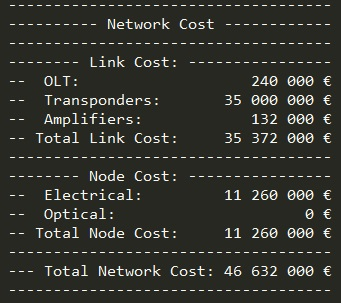
\includegraphics[width=9cm]{sdf/ilp/opaque_survivability/figures/script_opaque_surv_ref_medium}
\caption{The ILP script used in the medium scenario with the network cost.}
\label{scriptopaque_surv_ref_medium}
\end{figure}

As we can see the cost of CAPEX for this scenario is \textbf{100 580 000 \euro}.\\


\textbf{High Traffic Scenario:}\\

In this scenario we have to take into account the traffic calculated in \ref{high_traffic_scenario}. In table \ref{link_opaque_surv_ref_high} we can see the number of optical channels and the number of amplifiers for each link calculated through MatLab.

\begin{table}[h!]
\centering
\begin{tabular}{|| c | c | c ||}
 \hline
 \multicolumn{3}{|| c ||}{Information regarding LINK} \\
 \hline
 \hline
 Bidirectional Link & Optical Channels & Amplifiers\\
 \hline
 Node 1 <-> Node 2 & 1 & 4 \\
 Node 1 <-> Node 3 & 1 & 6 \\
 Node 2 <-> Node 3 & 1 & 0 \\
 Node 2 <-> Node 4 & 2 & 6 \\
 Node 3 <-> Node 5 & 1 & 8 \\
 Node 4 <-> Node 5 & 1 & 1 \\
 Node 4 <-> Node 6 & 2 & 7 \\
 Node 5 <-> Node 6 & 2 & 3 \\
 \hline
\end{tabular}
\caption{Table with information regarding Link}
\label{link_opaque_surv_ref_high}
\end{table}

In table \ref{node_opaque_surv_ref_high}  we can see the number of transceivers, the number of line ports and the number of tributary ports for each node.

\begin{table}[h!]
\centering
\begin{tabular}{|| c | c | c | c ||}
 \hline
 \multicolumn{4}{|| c ||}{Information regarding NODE} \\
 \hline
 \hline
 Node & Transceiver & Line Ports & Tributary Ports\\
 \hline
 1 & 2 & 2 & 29 \\
 2 & 3 & 4 & 23 \\
 3 & 3 & 3 & 18 \\
 4 & 3 & 5 & 20 \\
 5 & 3 & 4 & 24 \\
 6 & 2 & 4 & 22 \\
\hline
\end{tabular}
\caption{Table with information regarding Node}
\label{node_opaque_surv_ref_high}
\end{table}

Through the information obtained previously on the nodes we can now create tables with detailed information about each node.\\

\newpage
\begin{table}[h!]
\centering
\begin{tabular}{|| c | c ||}
 \hline
 \multicolumn{2}{|| c ||}{Detailed description of Node 1} \\
 \hline
 \hline
 \multirow{2}{*}{2 transceivers} & One to connect to Node 2 \\
  & One to connect to Node 3 \\ \hline
\multirow{2}{*}{2 line ports} & 1 line ports to connect to Node 2 \\
 & 1 line ports to connect to Node 3 \\ \hline
\multirow{3}{*}{29 tributary ports} & where 13 is the ODU0 \\
 & where 13 is the ODU1 \\
 & where 3 is the ODU2 \\
\hline
\end{tabular}
\caption{Table with detailed description of node 1}
\end{table}


\begin{table}[h!]
\centering
\begin{tabular}{|| c | c ||}
 \hline
 \multicolumn{2}{|| c ||}{Detailed description of Node 2} \\
 \hline
 \hline
 \multirow{3}{*}{3 transceivers} & One to connect to Node 1 \\
  & One to connect to Node 3 \\
  & One to connect to Node 4 \\ \hline
\multirow{3}{*}{4 line ports} & 1 line ports to connect to Node 1 \\
 & 1 line ports to connect to Node 3 \\
 & 2 line ports to connect to Node 4 \\ \hline
\multirow{5}{*}{23 tributary ports} & where 11 is the ODU0 \\
 & where 7 is the ODU1 \\
 & where 2 is the ODU2 \\
 & where 2 is the ODU3 \\
 & where 1 is the ODU4 \\
\hline
\end{tabular}
\caption{Table with detailed description of node 2}
\end{table}


\begin{table}[h!]
\centering
\begin{tabular}{|| c | c ||}
 \hline
 \multicolumn{2}{|| c ||}{Detailed description of Node 3} \\
 \hline
 \hline
 \multirow{3}{*}{3 transceivers} & One to connect to Node 1 \\
  & One to connect to Node 2 \\
  & One to connect to Node 5 \\ \hline
\multirow{3}{*}{3 line ports} & 1 line ports to connect to Node 1 \\
 & 1 line ports to connect to Node 2 \\
 & 1 line ports to connect to Node 5 \\ \hline
\multirow{4}{*}{18 tributary ports} & where 7 is the ODU0 \\
 & where 6 is the ODU1\\
 & where 3 is the ODU2\\
 & where 2 is the ODU3\\
\hline
\end{tabular}
\caption{Table with detailed description of node 3}
\end{table}

\newpage
\begin{table}[h!]
\centering
\begin{tabular}{|| c | c ||}
 \hline
 \multicolumn{2}{|| c ||}{Detailed description of Node 4} \\
 \hline
 \hline
 \multirow{3}{*}{3 transceivers} & One to connect to Node 2 \\
 & One to connect to Node 5 \\
 & One to connect to Node 6 \\ \hline
\multirow{3}{*}{5 line ports} & 2 line ports to connect to Node 2 \\
 & 1 line ports to connect to Node 5 \\
 & 2 line ports to connect to Node 6 \\ \hline
\multirow{3}{*}{20 tributary ports} & where 7 is the ODU0 \\
 & where 10 is the ODU1 \\
 & where 3 is the ODU2 \\
\hline
\end{tabular}
\caption{Table with detailed description of node 4}
\end{table}


\begin{table}[h!]
\centering
\begin{tabular}{|| c | c ||}
 \hline
 \multicolumn{2}{|| c ||}{Detailed description of Node 5} \\
 \hline
 \hline
 \multirow{3}{*}{3 transceivers} & One to connect to Node 3 \\
 & One to connect to Node 4 \\
 & One to connect to Node 6 \\ \hline
\multirow{3}{*}{4 line ports} & 1 line ports to connect to Node 3 \\
 & 1 line ports to connect to Node 4 \\
 & 2 line ports to connect to Node 6 \\ \hline
\multirow{5}{*}{24 tributary ports} & where 14 is the ODU0 \\
 & where 4 is the ODU1 \\
 & where 4 is the ODU2 \\
 & where 1 is the ODU3 \\
 & where 1 is the ODU4 \\
\hline
\end{tabular}
\caption{Table with detailed description of node 5}
\end{table}

\begin{table}[h!]
\centering
\begin{tabular}{|| c | c ||}
 \hline
 \multicolumn{2}{|| c ||}{Detailed description of Node 6} \\
 \hline
 \hline
 \multirow{2}{*}{2 transceivers} & One to connect to Node 4 \\
  & One to connect to Node 5 \\ \hline
\multirow{2}{*}{4 line ports} & 2 line ports to connect to Node 4 \\
 & 2 line ports to connect to Node 5 \\ \hline
\multirow{5}{*}{22 tributary ports} & where 8 is the ODU0 \\
 & where 10 is the ODU1 \\
 & where 1 is the ODU2 \\
 & where 1 is the ODU3 \\
 & where 2 is the ODU4 \\
\hline
\end{tabular}
\caption{Table with detailed description of node 6}
\end{table}


Now let's focus on the path information. These paths are bidirectional paths so the path from one node to another is the same path in the opposite direction. In table \ref{path_opaque_surv_ref_high} we can see all the paths obtained for all nodes.

\begin{table}[h!]
\centering
\begin{tabular}{|| c | c ||}
 \hline
 \multicolumn{2}{|| c ||}{Information regarding PATHS} \\
 \hline
 \hline
 Node1 <-> Node2 & -Link(1,2) \\
 Node1 <-> Node3 & -Link(1,3) \\
 Node1 <-> Node4 & -Link(1,2) -Link(2,4)\\
 Node1 <-> Node5 & -Link(1,3) -Link(3,5)\\
 Node1 <-> Node6 & -Link(1,3) -Link(3,5) -Link(5,6)\\
 Node2 <-> Node3 & -Link(2,3)\\
 Node2 <-> Node4 & -Link(2,4)\\
 Node2 <-> Node5 & -Link(2,3) -Link(3,5)\\
 Node2 <-> Node6 & -Link(2,4) -Link(4,6)\\
 Node3 <-> Node4 & -Link(3,2) -Link(2,4)\\
 Node3 <-> Node5 & -Link(3,5)\\
 Node3 <-> Node6 & -Link(3,5) -Link(5,6)\\
 Node4 <-> Node5 & -Link(4,5)\\
 Node4 <-> Node6 & -Link(4,6)\\
 Node5 <-> Node6 & -Link(5,6)\\
 \hline
\end{tabular}
\caption{Table with description of path}
\label{path_opaque_surv_ref_high}
\end{table}

Finally, through the figure \ref{scriptopaque_surv_ref_high} we can see the result of CAPEX obtained with this ILP model.

\begin{figure}[h!]
\centering
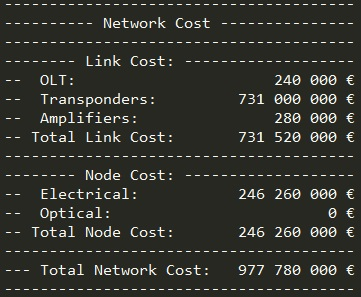
\includegraphics[width=9cm]{sdf/ilp/opaque_survivability/figures/script_opaque_surv_ref_high}
\caption{The ILP script used in the high scenario with the network cost.}
\label{scriptopaque_surv_ref_high}
\end{figure}

As we can see the cost of CAPEX for this scenario is \textbf{100 432 000 \euro}.